\documentclass[specification,annotation]{itmo-student-thesis}

%% Опции пакета:
%% - specification - если есть, генерируется задание, иначе не генерируется
%% - annotation - если есть, генерируется аннотация, иначе не генерируется
%% - times - делает все шрифтом Times New Roman, требует пакета pscyr.

%% Делает запятую в формулах более интеллектуальной, например: 
%% $1,5x$ будет читаться как полтора икса, а не один запятая пять иксов. 
%% Однако если написать $1, 5x$, то все будет как прежде.
\usepackage{icomma}



%% Данные пакеты необязательны к использованию в бакалаврских/магистерских
%% Они нужны для иллюстративных целей
%% Начало
\usepackage{tikz}
\usetikzlibrary{arrows}
\usepackage{filecontents}

%% Указываем файл с библиографией.
\addbibresource{bachelor-thesis.bib}

\begin{document}

\studygroup{M3439}
\title{Синтез исправлений для неверных решений олимпиадных задач по программированию}
\author{Шовкопляс Григорий Филиппович}{Шовкопляс Г.Ф.}
\supervisor{Буздалов Максим Викторович}{Буздалов М.В.}{канд. техн. наук}{доцент кафедры КТ Университета ИТМО}
\publishyear{2017}
%% Дата выдачи задания. Можно не указывать, тогда надо будет заполнить от руки.
\startdate{01}{сентября}{2017}
%% Срок сдачи студентом работы. Можно не указывать, тогда надо будет заполнить от руки.
\finishdate{31}{мая}{2017}
%% Дата защиты. Можно не указывать, тогда надо будет заполнить от руки.
%\defencedate{15}{июня}{2015}

%% Задание
%%% Техническое задание и исходные данные к работе
\technicalspec{Требуется разработать способ анализа кода программ для решения олимпиадных задач, 
с целью применения автоматического исправления ошибок
для повышения продуктивности обучения школьников. }

%%% Содержание выпускной квалификационной работы (перечень подлежащих разработке вопросов)
\plannedcontents{Пояснительная записка должна демонстрировать актуальность данной задачи и подход к решению.
Должна быть проведена оценка эффективности, а также оценены перспективы развития. }

%%% Исходные материалы и пособия 
\plannedsources{\begin{enumerate}
    \item ANTLR 4 Documentation;
    \item Томас Кормен и др. Алгоритмы: построение и анализ;
    \item Earl T. Barr, Mark Harman и др. Automated Software Transplantation.
\end{enumerate}}

%%% Календарный план
\addstage{Ознакомление с областью задачи, поиск существующих решений}{10.2017}
\addstage{Разработка алгоритма для решения задачи}{11.2017}
\addstage{Реализация алгоритма}{02.2017}
\addstage{Тестирование и оценка эффективности}{04.2017}
\addstage{Написание пояснительной записки}{05.2017}

%%% Цель исследования
\researchaim{Исследование возможности синтеза исправлений для неверных решений олимпиадных задач по программированию.}

%%% Задачи, решаемые в ВКР
\researchtargets{\begin{enumerate}
    \item Провести анализ актуальности;
    \item Разработать алгоритм для решения;
    \item Оценить эффективность алгоритма и возможности его улучшения.
\end{enumerate}}

%%% Использование современных пакетов компьютерных программ и технологий
\advancedtechnologyusage{Был использованы языки программирования Java 1.8, Python 3 и 
генератор ситаксических анализаторов ANTLR.
Для Java была добавлена библиотека StructureGraphic для визуализации деревьев, а также
библиотека для работы c ANTLR. Для разработки кода
использовалась среда Intellij IDEA c плагином для запуска ANTLR для написания кода на Java и 
FAR manager для написания кода на Python.}

%%% Краткая характеристика полученных результатов 
\researchsummary{Реализованный метод синтеза покрывает достаточно большое количество типичных ошибок,
а при дальнейшей доработке способен покрывать абсолютное большинство.}

%%% Гранты, полученные при выполнении работы 
\researchfunding{}

%%% Наличие публикаций и выступлений на конференциях по теме выпускной работы
\researchpublications{
}

%% Эта команда генерирует титульный лист и аннотацию.
\maketitle{Бакалавр}


%% Оглавление
\tableofcontents

%% Макрос для введения. Совместим со старым стилевиком.
\startprefacepage

В настоящее время популярны и продолжают набирать популярность различные олимпиады по программированию.
Особенностью данных олимпиад является использование автоматической системы тестирования, которая проверяет
программу участника на заранее подготовленных тестах.

Ведут работу и крайне востребованы различные кружки, онлайн-курсы и другие обучающие занятия в данной области.
Преподаватели постоянно ищут ошибки в программах учащихся в процессе обучения. Не всегда найти ошибку просто, 
особенно небольшую. 

При этом одну и ту же задачу решает множество различных школьников, в разные моменты времени, но все посылки
храняться на сервере с тестирующей системой в данном случае, в отличии от, например, математических задач,
которые чаще всего проверяются устно, либо письменно, но на бумаге, которую не хранят.

В любой области обучения можно столкнуться с ошибками, которые совершают множество людей при обучении,
в математике, например, это потеря корней при раскрытие модуля или деления на зависимую переменную.
Программирование не является исключением, и ошибки при решении задач тоже повторяются, однако, как описано выше
в рамках одной тестирующей системы хранится архив всех попыток сдач. 
Данную информацию как раз и хочется использовать, для повышения эффективности преподавания.

В данной работе будет рассмотрен способ синтеза исправлений для решения учащегося. Это поможет в некоторой
степени автоматизировать процесс обучения, а следовательно снять не самую полезную нагрузку с преподавателя.
Ведь, если в случае с локальным кружком на одного преподавателя приходится не более двадцати учащихся, но существуют
онлайн-курсы, в которых количество учащихся в разы больше. На заочном кружке Петра Калинина в год написания работы
обучалось $150$ человек на одного преподавателя. Но эти цифры меркнут на фоне количества учащихся на онлайн-курсе 
Максима Буздалова <<I2CPx>> за предыдущие два года суммарно достигло $60\,000$ человек. При этом, даже на 
такое огромное количество человек приходится всего один преподаватель.

В \textbf{первой} главе вводятся основные определения и термины, используемые в работе и необходимые
для понимания других определений и терминов. Также формулируется цель исследования, на основе которой
приводится обзор работ из смежных областей, после чего окончательно формулируется задача исследования.

В \textbf{второй} главе ...

В \textbf{третьей} главе ...


%% Начало содержательной части.
%% Начало содержательной части.
\chapter{Обзор области, постановка задачи}

\section{Термины и понятия}

В данном разделе описаны основные термины и понятия, используемые в представленной работе.

\subsection{Олимпиадное программирование}

\textbf{Задача} олимпиадного программирования представляет из себя некоторое задание, которое требуется выполнить, написав
программу на одном из языков программирования. Чтобы проверить корректность выполнения задания, текст программы
отправляют на проверку в тестирующую систему.

Под \textbf{тестирующей системой} в данной работе будем подразумевать сервер, на который учащиеся отправляют свой код, 
для проверки его корректного выполнения на заранее подготовленных тестах.

\textbf{Teст} для олимпиадной задачи по программированию~--- некоторые входные данные, удовлетворяющие условию задачи.
Как правило, представляет из себя текстовый файл. Для каждой задачи обычно существует свой набор тестов. В наборе может быть,
как один, так и несколько тестов. Тесты составляются до проведения соревнования или занятия и обычно неизвестны учащемуся.

\textbf{Решением} олимпиадной задачи называют программу, которая считывает входные данные, находит ответ и выводит его.
Также нередко в условии задачи присутствуют ограничения на время выполнения и количество используемой памяти, поэтому
корректное решение должно укладываться в эти ограничения.

\textbf{Вердикт} тестирующей системы~--- ответ тестирующей системы после проверки некоторого решения. 
Может быть положительным или одним из отрицательных. 
В случае получения положительного ответа, считается, что задача решена правильно, иначе, что в решении присутствует ошибка.
Как правило, вместе с вердиктом учащийся получает комментарий с номером теста, на котором решение работает некорректно.

\subsection{Ошибки в олимпиадном программировании}

\textbf{Ошибкой} будем называть причину, по которой решение получает отрицательный вердикт на одном из тестов.

Множество ошибок можно интуитивно разделить на несколько категорий:
\begin{enumerate}
    \item \textbf{Идейные}. Данные ошибки совершаются по причине написания неправильной интерпритации условия,
        либо некорректного выбора алгоритма для решения. Простой пример~--- решение задачи динамического программирования 
        о рюкзаке, используя метод жадного программирования. 
    \item \textbf{Неэффективный выбор алгоритма}. У некоторых алгоритмов бывают разные версии и модификации,
        поэтому бывает, что, например вместо реализации алгоритма Дейкстры с кучей, учащийся пишет 
        реализацию алгоритма Дейкстры без кучи. В подобных случаях решение выдает правильный ответ, но может
        либо потреблять памяти больше, чем указанное в условии максимальное доступное количество памяти
        либо не успевает завершиться раньше указанного в условии максимального времени работы.
    \item \textbf{Неаккуратная реализация} также является частой причиной нарушения ограничений работы.
        Например, в решении используется неоптимальный способ считывания входных данных, или неподходящая
        структура данных. Сюда же можно отнести обращения к незаалоцированной памяти и подобные ошибки.
        Основная причина таких ошибок, заключается в том, что учащийся придумал правильную идею решения, 
        выбрал правильный алгоритм, но не смог его корректно реализовать.  
    \item \textbf{Нерассмотренные случаи} часто приводят к отрицательным вердиктам. Во многих задачах существуют крайние случаи,
        например, когда в массиве один элемент и в этом случае программа будет работать некорректно. Лечатся такие ошибки при помощи
        условного оператора и отдельного рассмотрения этих самых случаев.
    \item \textbf{<<Мелкие>>} ошибки можно сравнить с помарками при решении математической задачи, на подобии потери знака при переносе.
        Такие ошибки легко допустить, но сложно заметить при самопроверке. В области олимпиадного программирования к таким ошибкам
        можно причислить неправильные типы, ошибки в индексации, неправильные размеры массивов. Особым отличием таких ошибок
        является то, что для того, чтобы помочь учащемуся, достаточно просто указать область кода, где она совершена, либо
        ограничится фразой по типу: <<У Вас ошибка в ограничениях в массиве>>, либо <<Нужно использовать 
        шестидесятичетырехбитный тип данных, вместо тридцатидвухбитного>>.   
\end{enumerate}


\subsection{Теория графов}

\textbf{Граф}~--- абстрактный математический объект, который характеризует 
пара $G = (V, E)$, где $V$~--- множество вершин, а $E \subset \{(v, u): v, u \in V\}$~--- множество ребер. 

\textbf{Связный граф}~--- граф, в котором между любой парой вершин существует хотя бы один путь.

\textbf{Цикл}~--- последовательность вершин вида $v_1, v_2 \dots v_k$, где $v_i \in V$, 
$(v_i, v_{i+1}) \in E$ и $v_1 = v_k$.

\textbf{Ациклический граф}~--- граф, который не содержит в себе циклов.

\textbf{Дерево}~--- связный ациклический граф.

В данной работе рассматриваются \textbf{подвешенные} деревья. Это деревья, у которых для каждых двух смежных по ребру
вершин выполняется отношение предок-потомок(по-другому родитель-ребенок).

Вершина, у которой нет потомков называется \textbf{листом}, в свою очередь вершина, у которой нет предков,
называется \textbf{корнем}. Очевидно, что у любого дерева ровно один корень, при этом листьев может быть сколько угодно много.

Рассмотрим некоторое дерево $T = (V, E)$. \textbf{Поддеревом} данного дерева будет дерево $T' = (V', E')$, такое что
$V' \subset V$ и $E' = \{(v, u) \in E : v, u \in V'\}$, при этом если $v \in V'$, то для любой
вершины $w$~--- потомок $v$ в дереве $T$, выполняется $w \in V'$

\textbf{Разностью} дерева $T = (V, E)$ и его поддерева $T' = (V', E')$ будем называть дерево $T'' = (V'', E'')$,
такое что $V'' = V \setminus V'$ и $E'' = \{(v, u) \in E : v, u \notin V'\}$. Интуитивно можно представить, что от дерева
$T$ <<отрезали>> его поддерево $T'$. Обозночать будем $T'' = T \setminus T'$.


\textbf{Поиск в глубину}~--- один из наиболее популярных алгоритмов обхода графа, используемый для изучения строения. 

\subsection{Синтаксический анализ}

\textbf{Абстрактное синтаксическое дерево} (дерево разбора)~--- структура данных, представляющая из себя ориентированное дерево, 
в котором каждая вершина сопоставляется с оператором языка программирования, а листья с соответствующими операндами. 

\textbf{Лексический анализ}~--- процесс аналитического разбора 
входного текста на известные группы, с последующем получением на выходе 
идентифицированных последовательностей, называемых <<токенами>>. 
Лексический анализ используется в компиляторах и интерпретаторах исходного кода языков программирования, 
и в различных парсерах слов естественных языков.

\textbf{Лексическим анализатором} (жарг. лексер от англ. $lexer$) называется программа, выполняющая лексический анализ текста.

\textbf{Синтаксический анализ}(жарг. парсинг от англ. $parsing$)~--- процесс сопоставления последовательности токенов(слов)
формального языка с его формальной грамматикой. Результатом будет абстрактное синтаксическое дерево. Как правило, для получения
токенов проводится лексический анализ.

\textbf{Синтаксическим анализатором} (жарг. парсер от англ. $parser$) называется программа выполняющая синтаксический анализ.

\textbf{Контекстно-свободная грамматика}~---  способ описания формального языка, в котором нет зависимости от контекста.

\textbf{Генератор синтаксических анализаторов}~--- программа, которая получает на вход контекстно-свободную грамматику 
некоторого языка, а на выход выдает синтезированный код лексического и синтаксического анализаторов для данного языка.
Для большинства используемых в олимпиадном программировании языков программирования 
существуют стандартные уже реализованные грамматики.

\section{Постановка цели исследования}
\subsection{Предпосылки}

Рассмотрим некоторый кружок, онлайн-курс или что-то подобное по олимпиадному программированию. 
В нем обучается некоторое количество учащихся, которых, как правило, многократно больше, чем преподавателей.

Процесс обучения включает в себя практику, которая представляет из себя решение олимпиадных задач, с последующей
отправкой решений на проверку в тестирующую систему. На каждую посылку решения, тестирующая система выдает некоторый вердикт.
В том случае, если вердикт положительный задача считается решенной правильно, и учащийся с чистой совестью переходит к решению
следующих задач, иначе же, учащийся будет пытаться самостоятельно найти ошибку.

Однако, как правило, большинство учащихся из-за лени, недостатка опыта, знаний или еще каких-либо причин не могут найти ошибку
самостоятельно и обращаются к преподавателю за помощью. Чтобы помочь в поиске ошибки, преподавателю необходимо прочитать код учащегося,
иногда не один раз, и потратить некоторое время. Когда подобных учащихся много, то и преподавательского времени тратиться 
непомерно много. Несложно предположить, что продуктивность преподавания можно повысить, если избавить преподавателя от 
подобных обязанностей путем автоматизации процесса.

Таким образом имеем базу предыдущих решений задачи с вердиктами, в том числе и с отрицательными, которые храняться в 
тестирующей системе. Хотим на основе этой информации, когда приходит новый запрос от учащегося на поиск ошибки, 
находить ее автоматически, если такая или подобная ей уже допускалась ранее другим участником. 

\subsection{Выбор фокусировки исследования}
В представленой работе будем фокусироваться именно на <<мелких>>, на что есть несколько достаточно веских причин:
\begin{itemize}
    \item Ошибки, не являющееся <<мелкими>> непонятно как именно находить, и скорее всего задача по поиску таких
        является NP-полной.
    \item Также, даже если представить, что мы нашли не являющуюся <<мелкой>> ошибку автоматически, неясно как
        компьютер сможет объяснить участнику, что же у него не так. Естественно фраза <<Замените вот тот код, на вот этот>>
        с приложенным следом кодом сомнительна, как минимум потому, что с таким же успехом, можно сказать <<вот правильный
        код, используйте его>>.
    \item Как было сказано выше, в случае <<мелкой>> ошибки, компьютер будет несложно научить давать комментарии, помогающие
        найти и исправить ее. 
    \item В случае поиска <<мелкой>> ошибки лично преподавателем, нужно прочитать
        весь код, иногда несколько раз. Именно на поиски таких ошибок, обычно, тратится наибольшее количество
        преподавательского времени.
    \item <<Мелкие>> ошибки чаще всего встречаются в коде, который нужно посмотреть преподавателю на предмет ошибок, 
        так как учащемуся проще их допустить, а также гораздо сложнее найти их самостоятельно.
    \item Такие ошибки также обладают свойством повторяться, ведь чем меньше размер кода представляющего ошибку, 
        тем больше вероятность, что подобную повторит кто-либо другой.
\end{itemize}


\section{Обзор смежной области}
Существуют несколько работ в смежных областях, цели которых чем-то похожи на поставленную в этой работы.

\subsection{Software transplantation}
Работа, которая на первый взгляд должна помочь в достижении поставленной цели~--- 
это <<Automated software transplantation>>~\cite{software-transplantation}.

В данной работе авторы рассматривают возможность <<пересадки>> кода из одной программы в другую, с целью передачи 
необходимой функциональности, по аналогии с трансплантацией огранов живого организма.

Для того, чтобы сделать это берется весь необходимый код, смотряться его зависимости от окружения и других частей программы, 
все это <<вырезается>> и ставится в код назначения в указанное место.

Несмотря на то, что метод зарекомендовал себя очень хорошо, работая в подовляющем большинстве тестовых случаев, применимо к поставленной
цели его использовать невозможно. Так как он попросту будет пересаживать код из правильного решения в неправильное и сообщать
что-то наподобии <<Я, конечно, не знаю, где у Вас ошибка, но если вы допишите в точности вот этот код, 
который раньше уже сдали в систему, то и Вы сдадите>>. Польза от данной информации, как уже было отмечено ранее крайне сомнительна,
да и в принципе ставит под вопрос необходимость использования таких сложных методов, лишь для того, чтобы показать учащемуся
правильный код, что, кстати, обычно, не делают, ведь теряется смысл обучения.

\subsection{Система поиска плагиата}
Имеет место идея применения парсеров и деревьев разбора, для поиска плагиата в текстах программ~\cite{anti-plagiat}.

Сравнения на плагиат в данной работе происходит ни непосредственно текста программы, а дерева разбора. Представленный
подход хорош тем, что сравнивает структуры программ, поэтому устойчив к переименованиям и переписыванием кода
с одного языка программирования на другой.

Также одной из особенностей работы является расширяемость за счет добавления новых грамматик на вход 
генератора синтаксических анализаторов. То есть, чтобы начать проверять новый язык программирования, надо
просто предоставить его грамматику.

Однако антиплагиат умеет лишь сравнивать два кода на похожесть по запрограммированной метрике, однако
он никак не может изменять программу, что для достижения поставленной цели в работе просто необходимо.
Также крупной проблемой является то, что в данном случае ищется именно плагиат, а в случае олимпиадного программирования
имеем один алгоритм реализованный двумя разными людьми, возможно, двумя абсолютно разными подходами.

Все же, возможность сравнивать отдельные части дерева разбора для сравнения их на похожесть~--- это идея,
которая найдет отражение в решении поставленной задачи.                                                                                                       

\subsection{Выводы по обзору смежной области}
К сожалению, ни одна из рассмотренных работ не помогает в достижении поставленной цели.
%других работ, которые были бы хотя бы настолько близки к поставленной задаче попросту не существует, 
%либо они не были найдены, несмотря на активные поиски автора. 
Что подводит к необходимости разработки своей системы синтеза
исправлений.


\section{Постановка задачи для исследования}
Основой исследования будут ранее сделанные изменения в коде решения, которые программа будет пробовать применить к текущему решению,
в котором требуется исправить ошибку. В этом разделе речь пойдет про решения по одной конкретной задаче.

Рассмотрим два решения некоторого участника, который ранее получил положительный вердикт, по интересующей нас задаче.
При этом первое решение из рассматриваемых получило отрицательный вердикт, а второе либо положительный, либо отрицательный, но
на более высоком номере теста. Важно, чтобы второе решение, было позже в хронологическом порядке, интересны именно изменения, которые
привели к улучшению вердикта.

Затем рассмотрим деревья разбора для кода двух выбранных решений. Дерево разбора первого решения назовем $A$, второго~--- $B$.
\textbf{Исправлением} назовем пару $(C_1, C_2)$, где $C_1$~--- поддерево дерева $A$, $C_2$~--- поддерево дерева $B$,
при этом $A \setminus C_1 = B \setminus C_2$. Интуитивно исправление представляется следующим образом: из первого решения
удалили отрывок кода, который сопоставлялся дереву разбора $C_1$, а вместо него написали отрывок кода, сопоставляющийся $C_2$,
получив таким  образом второе решение. С точки зрения деревьев, одно поддерево было заменено на другое.

По определению исправление улучшает вердикт для решения задачи. Под \textbf{опытом} будем подразумевать известные исправления.

Пусть теперь мы получили новое решение учащегося, в котором нужно найти ошибку. Также знаем для него вердикт тестирующей системы. 
Рассмотрим все прошлые исправления $(C_1, C_2)$ по данной задаче, после чего попробуем применить его уже к новому решению. 
Для этого в дереве разбора нового решения необходимо найти поддерево <<похожее>> на $C_1$, заменить его на поддерево
<<похожее>> на $C_2$, а затем проверить подошло исправление или нет. Будем считать его подходящим, если при отправке
получившегося кода в тестирующую систему вердикт будет лучше, чем полученный ранее.

Таким образом, можно по пунктам сформулировать окончательную задачу для исследования:
\begin{itemize}
    \item Выбрать метод анализа деревьев разбора программ.
    \item Научиться находить исправление по двум разным версиям одного решения.
    \item Сформулировать критерий <<похожести>> двух поддеревьев.
    \item Научиться применять исправление.
    \item Проверить исправление на улучшение вердикта.
    \item Оценить эффективность и предложить пути улучшения.
\end{itemize}

\chapterconclusion

\begin{enumerate}
    \item Введены необходимые термины и определения.
    \item Установлено, что существующие методы работы с кодом, не применимы для решения задачи синтеза исправлений 
        в олимпиадной задаче по программированию.
    \item Сформулирована цель и задача исследования выпускной квалификационной работы.
\end{enumerate}

\chapter{Решение поставленной задачи}

\section{Анализ текста решения}

\subsection{ANTLR}
Для синтаксического анализа решения предлагается использовать генератор анализаторов для формальных языков ANTLR.
Чтобы получить парсер нужного языка, достаточно просто передать грамматику для данного языка в нужном формате.
ANTLR зарекомендовал себя как стабильное и удобное средство для работы с синтаксическим анализом, при этом
обладая крайне полезными для представленной работы приемуществами:
\begin{itemize}
    \item Свободное программное обеспечение.
    \item Использование единой нотации для описания лексических и синтаксических анализаторов.
    \item В репозитории разработчиков есть примеры грамматик для многих популярных языков программирования.
    \item Множество плагинов для работы в различных средах разработки, в том числе и для Intellij IDEA, которая
        использовалась в данной работе.
    \item Возможность добавлять Java-код в грамматику с целью подстановки его напрямую в парсер. При помощи этого 
        можно запрограммировать парсер возвращать какую-угодно информацию о тексте.
    \item Предоставление сообщений об ошибках и восстановление после них, в том числе корректная обработка отсутствующих узлов, 
        с последующим продолжением работы над остальным текстом. 
\end{itemize} 

Основной сложностью при работе с ANTLR стало то, что он не умеет по дереву разбора восстанавливать исходный код программы, так
как все пробелы и разделители убираются при работе лексера, и никаких обратных приобразователей не генерируется. Также проблемой
стало отсутствие возможности как-либо модифицировать построенные деревья разбора, однако обе эти проблемы решаемы.

Чтобы решить возникшие проблемы, можно модифицировать стандартную реализованную грамматику из репозитория разработчиков
добавив код, который будет строить дерево разбора, методы и структуру для которого можно реализовать отдельно на языке
Java.

После модификации грамматики работа с ANTLR сводится к нажатию пары кнопок для генерации лексера и парсера. 

\subsection{Выбор языка программирования}

Так как работать планируется со структурой кода при помощи деревьев разбора, можно не умаляя общности рассматривать один
конкретный язык программирования. Для добавления другого языка нужно будет лишь использовав новую грамматику получить новые лексер
и парсер, а также запрограммировать элементы структуры дерева разбора.

В данной работе будет рассматриваться язык программирования Паскаль. Это один из наиболее популярных языков для олимпиад
по программированию, который долгое время использовался для начального обучения школьников и студентов. В момент написания
работы, язык программирования сдал лидирующие позиции, однако все еще популярен и используется даже на всероссийской олимпиаде
школьников по программированию (РОИ). Язык дорабатывается по сей день в рамках языков Pascal ABC и Delphi.

Паскаль имеет следующие оссобенности:
\begin{itemize}
    \item Строгая типизация.
    \item Структурное программирование.
    \item Текстовая простота.
\end{itemize}

При программировании на Паскале может сложиться ощущение, что вы программируете на английском языке, настолько синтаксис оптимизирован
для обучения.

В представленной работе будет рассмотрено избыточное подмножество изначального стандарта языка 
<<Pascal Standard>>, принятого в 1974 году.

\begin{algorithm}[!h] 
\caption{Пример программы на языке Паскаль}\label{lst1} 
\begin{lstlisting}[language=pascal]
program tmp;
const
  Author = 'Grigory';
var
  arr: array[1..2] of string;
begin
  writeln('Hi')
end.
\end{lstlisting} 
\end{algorithm}

\subsection{Дерево разбора}

Для работы с деревьями разбора по причинам, описанным ранее, необходимо было разработать собственную структуру данных, представляющую
дерево разбора, при этом позволяющую изменять свою структуру и получать код программы, которой это дерево отвечает.

Разработка данной структуры проводилась на языке программирования Java. Этот язык объектно ориентированный, что положительно сказалось
на дизайне кода и удобстве его написания, а также ANTLR, как уже отмечалось, отлично с ним совместим.

Структура данных наследуется из основного общего класса \texttt{ASTNode}, который представляет из себя вершину дерева.
Основные типы вершин это:
\begin{itemize}
    \item переменная;
    \item константа;
    \item функция;
    \item процедура;
    \item условие;
    \item цикл с предусловием;
    \item цикл с постусловием; 
    \item цикл со счетчиком;
    \item перечисление (код между \texttt{begin} и \texttt{end});
    \item текст;
    \item тип.
\end{itemize}
Также есть вспомогательные:
\begin{itemize}
    \item двоичная операция;
    \item унарная операция;
    \item скобки;
    \item строка;
    \item универсальная.
\end{itemize}

Универсальная вершина разработана для удобства, через вершину данного типа можно разработать любую вершину, у которой есть дети.
От нее наследуются, например, вершины двоичной и унарной операций, а также вершиана перечислений.  

Данная структура предназначена для представления конкретно выбранного языка, но несложно дополняется для поддержки дополнительной
функциональности языка, либо другого языка.

\begin{figure}[!h] 
\caption{Пример дерева разбора для программы из листинга~\ref{lst1}}\label{fig1} 
\begin{center}
  \makebox[\textwidth]{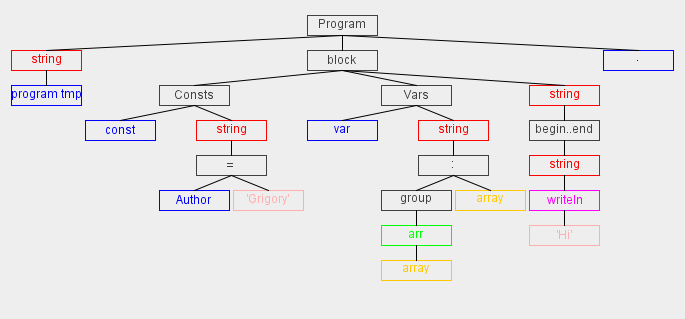
\includegraphics[width=0.9\paperwidth]{pics/tree-example.png}}
\end{center}
\end{figure}

Как было отмечено ранее, ANTLR поддерживает вставки Java-кода, поэтому стандартная грамматика была модифицирована для поддержки
разработанной структуры данных. Пример приведен в листинге~\ref{lst2}. 

\begin{algorithm}[!h] 
\caption{Пример грамматики ANTLR с вставками Java-кода}\label{lst2} 
\begin{lstlisting}[basicstyle=\small] 
constant returns [ASTNode ast]
 :unsignedNumber {
   $ast = new ConstNode($unsignedNumber.text, "num");
  }
 |sign unsignedNumber {
   $ast = new ConstNode($sign.text + $unsignedNumber.text, "sNum");
  }
 |identifier {
   $ast = new ConstNode($identifier.text, "id");
  }
 |sign identifier {
   $ast = new ConstNode($sign.text + $identifier.text, "sId");
  }
 |string {
   $ast = new ConstNode($string.text, "str");
  }
 ; 
\end{lstlisting} 
\end{algorithm}

В представленной структуре для каждого поддерева реализован метод \texttt{toString}, который сопоставляет ему
корректный код программы, который репрезентует данное поддерево. 

\section{Работа с деревьями разбора}

\subsection{Поиск исправления}

Имеется два решения участника. Построим для них деревья разбора, представленные структурой данных, описанной выше, 
с помощью имеющегося парсера. Также вспомним, что 

\chapterconclusion

\begin{enumerate}
    \item ...
\end{enumerate}


\printmainbibliography

\end{document}
